
As \emph{Redes Neurais Artificiais} (RNAs) são uma tentativa computacional de modelar a capacidade de processamento de informação do sistema nervoso humano \cite{rojas}. Para alcançarem um bom desempenho, as RNAs empregam uma interligação de estruturas bases chamadas de neurônios artificiais que, por sua vez, possuem pesos com valores numéricos positivos ou negativos associados entre si. Uma vantagem das RNAs é a grande capacidade de generalização, ou seja, a habilidade de produzir saídas adequadas para entradas que não estavam presente anteriormente durante seu aprendizado \cite{haykin}. As RNAs têm sido frequentemente aplicadas nas áreas de medicina e negócios, além de um frequente desenvolvimento nos campos de processamento de sinais, reconhecimento de padrões em imagens e reconhecimento e produção de fala \cite{fausett}.

A idealização dos neurônios artificiais foi inspirada nos neurônios biológicos encontrados no cérebro humano. Como mostrado na Figura \ref{fig:neuronio}, cada neurônio biológico é composto pelo corpo celular, os dendritos e o axônio. Os dendritos têm como papel a recepção das informações, ou impulsos nervosos, de outros neurônios e a submissão destas informações ao corpo celular, onde são processadas e novos impulsos são gerados. Estes impulsos são enviados aos dendritos de outros neurônios através do axônio. O ponto de contato entre os neurônios através do axônio e os dentritos, denominado sinapse, é onde ocorre toda a troca de informação necessária para conceber uma rede neural \cite{braga}.

% Procurar nova imagem
\begin{figure}[h!]
\centering
\caption{Estrutura de um neurônio biológico. Adaptado de: \cite{braga}}
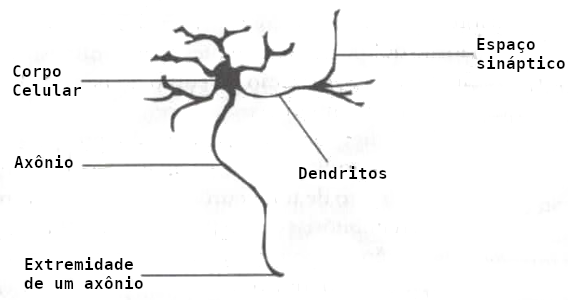
\includegraphics[width=0.6\textwidth]{imgs/neuronio}
\label{fig:neuronio}
\end{figure}

Considerando uma analogia com os neurônios biológicos, modelou-se então a primeira noção de neurônios artificiais. Nestes neurônios, as entradas são valores $x = x_1, ..., x_n$ aos quais estão sujeitos um conjunto de pesos $w = w_1, ..., w_n$. Este modelo de neurônio utiliza ainda um \emph{bias} externo, denotado por $b$. Este bias é utilizado para o aumentar ou diminuir os valores de entrada da função de ativação, dependendo se o seu valor é positivo ou negativo, respectivamente \cite{haykin}. Um neurônio artificial dispara quando a soma ponderada da entrada e do \emph{bias} sujeita aos pesos ultrapassa um certo limiar de excitação, denominado \emph{threshold}. No modelo de neurônio artificial apresentado, proposto por McCulloch e Pitts (MCP) \cite{mcculloch}, a ativação (disparo) do neurônio é obtida através da aplicação de uma \emph{função de ativação}, como mostrado na Figura \ref{fig:neuronio-artificial} \cite{braga}.

\begin{figure}[H]
\centering
\caption{Representação de um neurônio artificial. Adaptado de: \cite{haykin}.}
\label{fig:neuronio-artificial}
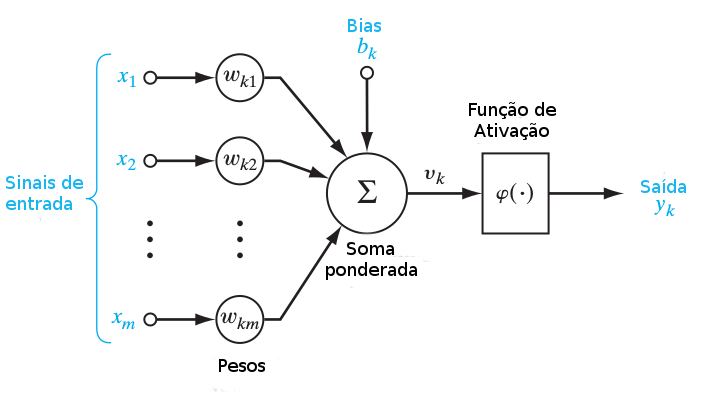
\includegraphics[width=0.8\textwidth]{imgs/neuronio-artificial}
\end{figure}

No caso do neurônio MCP, a função de ativação é do tipo degrau deslocada, conforme Equação \ref{eq:degrau}, e o seu valor de saída é obtido como resultado da comparação entre o \emph{threshold} $\theta$ previamente definido e o valor da soma ponderada da entrada, como mostrado na Equação \ref{eq:soma-ponderada}.

\begin{equation}
\label{eq:degrau}
\varphi(v) = \left\{
\begin{array}{lr}
  1, & \text{se } v > \theta.\\
  0, & \text{caso contrário}.
\end{array}
\right.
\end{equation}

\begin{equation}
  \label{eq:soma-ponderada}
  v = \sum\limits_{i=1}^n x_i w_i + b
\end{equation}


%%Para a correta funcionalidade de determinados algoritmos em RNAs, como o de \emph{backpropagation} em redes \emph{multilayer perceptron}, sabe-se que a escolha da função de ativação deve considerar funções contínuas e diferenciáveis \cite{haykin}.

Embora o modelo MCP tenha considerado apenas funções de ativação do tipo degrau deslocada, outras definições também são possíveis. As funções identidade, sigmóide, tangente hiperbólica e retificada linear (ReLU) são comumente utilizadas, definidas tais como mostrado na Figura \ref{fig:activation}.

\begin{figure}[h!]
  \caption{Exemplos de funções de ativação.}
  \label{fig:activation}
     \subfloat[Identidade ou Linear\label{subfig:identity}]{%
       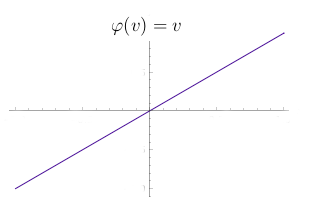
\includegraphics[width=0.4\textwidth]{imgs/identity}
     }
     \hfill
     \subfloat[Tangente Hiperbólica\label{subfig:tanh}]{%
       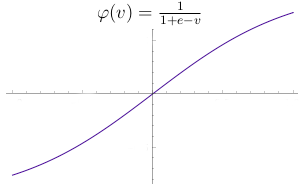
\includegraphics[width=0.4\textwidth]{imgs/tanh}
     }
     \hfill
     \subfloat[Sigmóide ou Logística\label{subfig:sigmoid}]{%
       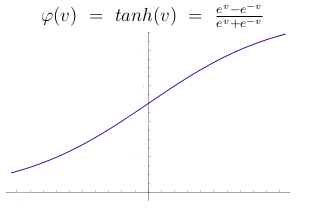
\includegraphics[width=0.4\textwidth]{imgs/sigmoid}
     }
     \hfill
     \subfloat[Unidade Linear Retificada (ReLu)\label{subfig:relu}]{%
       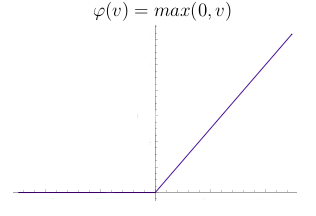
\includegraphics[width=0.4\textwidth]{imgs/relu}
     }
\end{figure}


Em 1958, visando a melhoria do neurônio MCP, Frank Rosenblatt desenvolveu o modelo \emph{Perceptron} \cite{Rosenblatt}. Neste modelo, criou-se o primeiro conceito de aprendizado através de neurônios artificiais, em que foi projetada uma regra de correção de erros para modificar os pesos associados a um neurônio quando suas respostas aos estímulos apresentados ao modelo forem erradas \cite{arbib}. Durante o processo de adaptação à resposta real, deseja-se identificar um valor $\Delta w$ a ser aplicado ao vetor de pesos atual $w(t)$, para que seu valor atualizado $w(t+1)$ esteja mais próximo da solução desejada do que o valor atual $w(t)$. Para isso, definiu-se a Equação \ref{eq:aprendizado1}, denominada Regra Delta, cuja obtenção, descrita na Equação \label{eq:aprendizado2} estabelece o modo detalhado como esse ajuste de pesos é efetuado. Nesta segunda equação, $\eta$ indica uma \emph{taxa de aprendizado}, isto é, a velocidade em que o vetor de pesos será atualizado, e $\hat{y}(t)$ significa o valor previsto pelo modelo naquela iteração para a entrada $x(t)$, enquanto $y(t)$ refere-se à saída real para esta entrada. Desta forma, o neurônio Perceptron adquiriu a capacidade de resolver problemas linearmente separáveis \cite{braga}.

\begin{eqnarray}
  w(t+1) &=& w(t) + \Delta w   \label{eq:aprendizado1}\\
  &=& w(t) + \eta (y - \hat{y}) x(t) \label{eq:aprendizado2}.
\end{eqnarray}

% Arquitetura das redes neurais.
Neurônios artificiais possuem uma capacidade de generalização limitada, independente da função de ativação escolhida, devido a sua habilidade de resolver apenas problemas linearmente separáveis. Entretanto, a combinação desses neurônios para a formação de uma rede é capaz de resolver problemas de elevada complexidade \cite{braga}. Geralmente, identificam-se três classes fundamentais de RNAs, as \emph{feedforward} com uma única camada, as \emph{feedforward} com múltiplas camadas e as recorrentes. Numa rede do tipo \emph{feedforward}, como as mostradas nas Figuras \ref{subfig:singlelayer} e \ref{subfig:multilayer}, existe uma camada de entrada que é projetada diretamente para uma camada de saída constituída de neurônios, e nunca ao contrário. Uma rede recorrente, como a na Figura \ref{subfig:recurrent}, por sua vez, possui conexões ponderadas dentro de uma camada e diferencia-se pela presença de pelo menos um loop de retorno a camadas anteriores. Esses loops de retorno possuem ainda um retardo de uma unidade de tempo aplicado ao vetor de saída, denotado por $z^{-1}$ \cite{haykin}.

% Inserir imagem da topologia das redes com subfig. Haykin ou Faceli.

\begin{figure}[h!]
  \caption{Arquiteturas populares de RNAs. Fonte: \cite{haykin}}
  \centering
     \subfloat[\emph{Feedforward} com uma única camada\label{subfig:singlelayer}]{%
       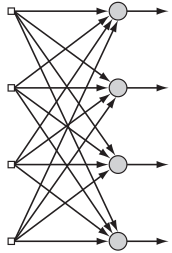
\includegraphics[width=0.25\textwidth]{imgs/feedforward-single}
     }
     \hfill
     \subfloat[\emph{Feedforward} com múltiplas camadas\label{subfig:multilayer}]{%
       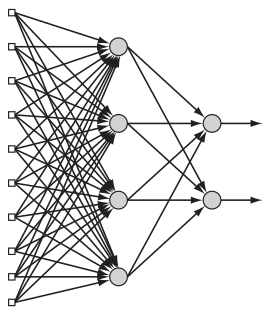
\includegraphics[width=0.35\textwidth]{imgs/feedforward-multi}
     }
     \hfill
     \subfloat[Recorrente\label{subfig:recurrent}]{%
       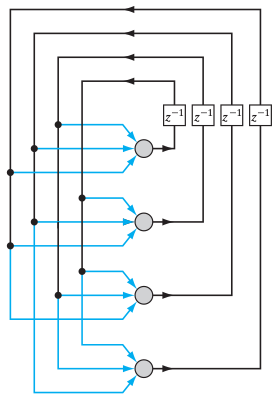
\includegraphics[width=0.3\textwidth]{imgs/recurrent}
     }
     \label{fig:architectures}
\end{figure}

Redes com múltiplas camadas, como na Figura \ref{subfig:multilayer}, caracterizam-se pela presença de pelo menos uma camada oculta. Isso acarreta um grande poder às redes deste tipo pois, conforme Cybenko, uma rede com uma camada oculta é capaz de mapear qualquer função contínua, enquanto uma rede com duas camadas ocultas é suficiente para mapear qualquer função \cite{cybenko}.

\subsubsection{\emph{Multilayer Perceptron}}
\label{subsubsec:mlp}

As RNAs do tipo \emph{Multilayer Perceptron} (MLP), são redes constituídas do neurônio Perceptron, \emph{feedforward} e com múltiplas camadas, sendo estas uma camada de entrada, uma ou mais camadas ocultas e uma camada de saída. A arquitetura mais comum para uma rede MLP é a completamente conectada, de forma que os neurônios de uma camada estão conectados a todos os neurônios da próxima camada \cite{faceli}.

Em uma rede MLP, a função implementada por um neurônio de certa camada é uma combinação das funções realizadas pelos neurônios da camada anterior que estão conectados a ele. Na primeira camada, cada neurônio aprende uma função que define um hiperplano. Na camada seguinte, os neurônios combinam um grupo de hiperplanos, formando regiões convexas. Os neurônios da camada seguinte combinam então um subconjunto das regiões convexas em regiões de formato arbitrário \cite{faceli}. Na Figura \ref{fig:aprendizado-mlp}, tem-se uma visualização do processo ocorrido.


\begin{figure}[h!]
\centering
\caption{Papel exercido pelos neurônios em cada camada de uma rede MLP. Fonte: \cite{faceli}.}
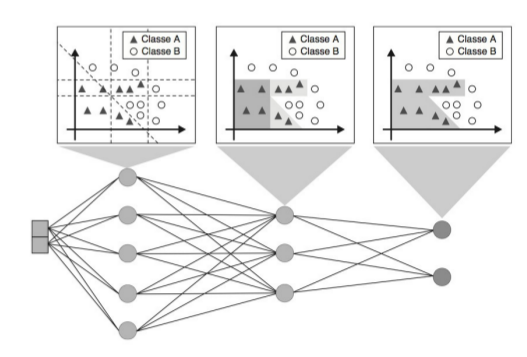
\includegraphics[width=0.7\textwidth]{imgs/aprendizado-mlp}
\label{fig:aprendizado-mlp}
\end{figure}

\todo{inserir informação sobre a necessidade de uma função de ativação contínua e diferenciável para o uso de backpropagation}
O algoritmo de aprendizado supervisionado mais conhecido e utilizado para treinamento das MLPs é o \emph{backpropagation}. Neste algoritmo utiliza-se as entradas e as saídas desejadas para o ajuste dos erros da rede. O treinamento ocorre em duas fases, a fase \emph{forward} e a fase \emph{backward}, em que cada fase percorre a rede em um sentido. Na fase \emph{forward}, a saída da rede é definida considerando certo padrão de entrada. A fase \emph{backward} utiliza a saída desejada e a saída fornecida pela rede para atualizar os pesos nas suas conexões \cite{braga}. O \emph{backpropagation} é simplesmente um método que utiliza o gradiente descendente para minimizar o erro total da saída calculada pela rede, na qual a derivada parcial define o ajuste dos pesos. Essa derivada mede a contribuição de cada peso no erro da rede para a classificação de dado objeto \cite{fausett, faceli}.

No âmbito do cálculo, o gradiente indica o sentido e a direção para os quais devem-se mover os valores dos pesos e do bias nas camadas, de forma a garantir o maior incremento possível de perda. Ou seja, nas técnicas de \emph{backpropagation}, queremos mudanças de peso que trarão a inclinação mais íngreme ao longo da função de erro, com o intuito de encontrar o mínimo global desta função \cite{goodfellow, kubat}.

Um grande crescimento do poder computacional em termos de velocidade e memória tem acontecido nos últimos tempos. Dado isto, houve a viabilidade de treinamento das chamadas \emph{redes neurais profundas}, MLPs que possuem mais camadas escondidas do que o usual. Devido a ampla popularidade dessas redes e a capacidade computacional para a utilização de grande quantidade de dados de treinamento, foram desenvolvidas técnicas de \emph{deep learning} em pleno estado da arte para detecção, segmentação, classificação e reconhecimento de objetos em imagens \cite{khan}. Utilizando-se redes neurais convolucionais, podemos ainda elencar aplicações como o reconhecimento de padrões em imagens para uso na medicina \cite{cha}, a modelagem de frases por computadores \cite{kalchbrenner} e o reconhecimento de caracteres e dígitos \cite{lecun}. Essas e outras técnicas serão apresentadas mais profundamente nas seções a seguir.

%%%%%
